\documentclass[tikz]{standalone}
\usepackage{tikz}

\begin{document}    
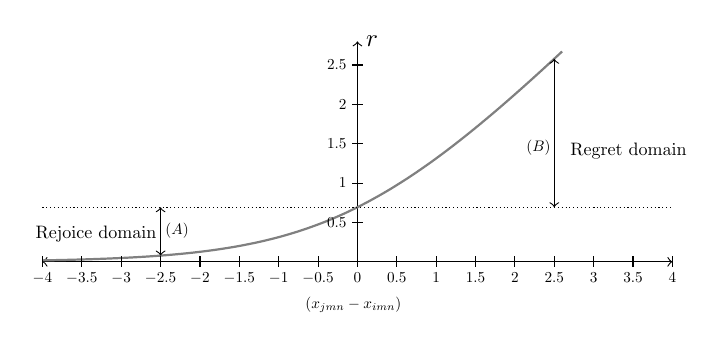
\begin{tikzpicture}
 \usetikzlibrary{positioning}
 \node (center) {};
 
 
 %Coordinates
 \coordinate (RRMcoordinate) at (0.5,1);

 
 %Name

  \node (rejoice) [scale=0.65,above right=1.1cm and 2.5cm of center,black ] {Regret domain};
 % \node (rejoice) [scale=0.55,above right=0.1cm and 2.5cm of center,red ] {Rejoice domain};
 % \node (rejoice) [scale=0.55,above left=1cm and 2.5cm of center ,red ] {Regret domain};
  \node (rejoice) [scale=0.65,above left=0.05cm and 2.35cm of center,black ] {Rejoice domain};
 
 
 \node (rejoice-2) [scale=0.55,above right=1.15cm and 1.95cm of center,thick ] {$(B)$};
  \node (rejoice) [scale=0.55,above left=0.1cm and 1.95cm of center ] {$(A)$};
 
 
 
 
 %Axis
   \draw[<->] (-4, 0) -- (4, 0) node[scale=0.55,below left= 0.25cm and -.75cm of center] {$(x_{jmn} - x_{imn})$};
  \draw[->] (0,0 ) -- (0, 2.8) node[right,scale=0.9] {$r$};
  
 %Functions 

   \draw[scale=1, domain=-4:2.6, smooth ,variable=\x, gray,thick] plot  ({\x}, {ln(1+exp(\x))});
  %\draw[scale=1, domain=-2.1:4, smooth ,variable=\x, red,thick] plot  ({\x}, {ln(1+exp(-\x))});
  \draw[scale=1, domain=-4:4, densely dotted ,variable=\x, black] plot  ({\x}, {ln(2)});

% Rejoy/regret lines
  \draw[<->,scale=1, domain={ln(2)}:{ln(1+exp(2.5))}, smooth ,variable=\x, black] plot  (2.5,{\x} );
  \draw[<->,scale=1, domain={ln(2)}:{ln(1+exp(-2.5))}, smooth ,variable=\x, black] plot  (-2.5,{\x} );



 \foreach \x/\xtext in {0,0.5,1,1.5,2,2.5,3,3.5,4}
\draw[shift={(\x,0)}] (0pt,2pt) -- (0pt,-2pt) node[scale=0.55,below] {$\xtext$};

 \foreach \x/\xtext in {0.5,1,1.5,2,2.5,3,3.5,4}
\draw[shift={(-\x,0)}] (0pt,2pt) -- (0pt,-2pt) node[scale=0.55,below] {$-\xtext$};

  \foreach \y/\ytext in {0.5,1,1.5,2,2.5}
  \draw[shift={(0,\y)}] (2pt,0pt) -- (-2pt,0pt) node[scale=0.55,left] {$\ytext$};
  %Labels of functions


 % \draw[->] (RRM) -- (RRMcoordinate);

  
\end{tikzpicture}
\end{document}


